\chapter{Current APIs\label{section:currentAPIs}}
\textbf{TODO: create high level diagrams of the other APIs}

In this chapter we will first give an overview of what APIs are available for
use, after which we will compare the APIs with features, finally covering
feature differences and performance statistics. Unfortunately there are no
direct statistics that show how much each API is used. Some were gathered
through interviews, although the sample size is not large enough to say
conclusively whether one is used more or another.

There is an additional camera API from Nvidia that we will not cover, namely
SIPL. This requires Nvidia specific hardware that is not easy to acquire. The
main difference with it is that it is a streaming based API that is safety
certified\footnote{\href{https://developer.nvidia.com/docs/drive/drive-os/6.0.8.1/public/drive-os-linux-sdk/common/topics/nvmedia\_concept\_nvsipl/PlatformCameraConfiguration.html}{developer.nvidia.com}},
meaning it can be used in automotive.

\section{Introduction to camera APIs}
\subsection{Video For Linux 2}\label{section:v4l2}
\textit{Video For Linux 2} (V4L2) serves as the fundamental low-level API
within Linux\footnote{https://www.kernel.org/doc/html/v4.9/media/intro.html}.
It is designed for managing video capture and output devices (among other things
like radio). It serves as the foundation for many of the higher-level APIs that
offer more user friendly approaches for video processing. V4L2 uses a very
minimalist approach, providing the user with great control over the camera
devices, with standard ways to control almost any camera device.

V4L2 is a very low level API, it does not provide any of the convenience
features found  in modern APIs. This allows V4L2 to have a very intricate
control over the camera, though requiring more management by the developer.
Being a C api, there are few encapsulating structures for things like images.
Instead everything is treated as buffers that the user must manage directly,
this can lead to more complexity and potential errors as developers are known
to not be very good at this~\cite{van2012memory}. The camera is controlled
using \textit{ioctl} commands. \textit{ioctl} commands are ways to configure
devices that normally are not configurable by file operations directly.

V4L2 still is widely used in fields such as robotics\footnote{Personal
communication, October 2024}, although hopefully we will move away from it once
libraries like Argus and libcamera gain traction.

V4L2 is split into two libraries, the kernel side which is known as V4L2, and the
userspace library known as libv4l2. The userspace library often just wraps the
kernel functions and forwards the arguments to the kernel API.

In \cref{appendix:section:v4l2} we can see an example of how to capture an
image using V4L2. This sample code is the most basic example where the camera
captures a single image into \textit{out.ppm}\footnote{In order to view this
image install a program such as \textit{feh}}. While the API is quite simple
considering most C APIs, it is still much more complex than the other APIs
where it is much clearer when you capture the image.

\subsection{Argus}\label{section:argus}
%https://docs.nvidia.com/jetson/l4t-multimedia/group__LibargusAPI.html
\begin{figure}
    \begin{center}
        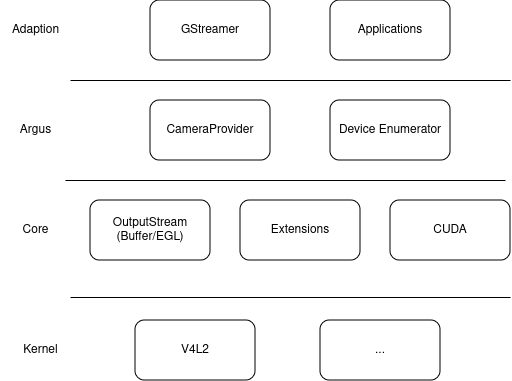
\includegraphics[width=0.55\textwidth]{figures/argus.png}
    \end{center}
    \caption{A block diagram of Argus}\label{fig:argusblock}
\end{figure}


Argus\footnote{https://docs.nvidia.com/jetson/l4t-multimedia/group\_\_LibargusAPI.html}
is a camera API that is developed by Nvidia. Argus runs only on Nvidia
hardware, such as the Jetson Orin Nano Developer Kit. While the API is
proprietary, this chapter aims to give an overview of how the API works and
fits into the grand scheme of things.

Argus is roughly based on V4L2 though effectively a re-implementation\footnote{Personal communication, Laurent Pitchard, 2024}.
At the time Argus was created, V4L2 was still in an early stage. It did not
supporting a variety of features such as multicamera setups etc. hence Argus
was created in order to add the missing features easily. These days V4L2 and
Argus are very close though in later chapters we will give an overview of what
pros and cons each has.

The reason Argus does not use V4L2 is largely a historical one at this point.
At the time Argus was created V4L2 was in an early stage, it had very limited
features. Nvidia created Argus in order to leviate these issues but ended up
with an API that is very similar to V4L2. Automotive for example needed support
for multi camera use cases, this was something that was not supported in V4L2 at
the time.

Over time, the API has aged a little though. Today it is still very dependent
on EGL. Like OpenGL, EGL is a very old API, today it does not receive many
updates. Effectively only when requested by big customers, even then it is
almost exclusively to enable emulation using Vulkan\footnote{Tony Zlatinski,
Personal communication, October 2024}. The issue with OpenGL and EGL is that it
assumes an internal state. While this state allows users to create applications
quickly, avoiding much boilerplate, it also sets a "glass ceiling". This
ceiling sets a limit on how fast applications can run as certain things can not
be optimized. This is why Vulkan was created, to allow the developer to specify
everything, though requiring more work to set up.

In \cref{fig:argusblock} we can see a block diagram of how Argus roughly works.
It has quite a similar architecture as libcamera (as seen in
\cref{fig:libcameraarch}), the main difference is that there are no IPAs that
are exposed to the user as these are trade secrets. The algorithms are provided
to the user as is, the autocontrol algorithms can be configured through the
\textit{Request} class where the settings are specified.

Through the use of EGLStreams, Argus is able to do zero-copy output to for
displays and encoders\footnote{https://docs.nvidia.com/jetson/l4t-multimedia/l4t\_mm\_10\_camera\_recording.html}.

The capture process in Argus is highly structured and optimized for
performance, leveraging NVIDIA’s hardware capabilities. It begins with the
creation of a \textit{CameraProvider} object, which serves as the entry point
to the Argus API. The \textit{CameraProvider} enumerates all available camera
devices on the system and provides access to them through
\textit{CameraDevice} objects. Each \textit{CameraDevice} represents a
physical or virtual camera in the system.

Once a specific \textit{CameraDevice} is selected, a \textit{CaptureSession} is
created through the \textit{ICaptureSession} interface. This session manages
all capture operations and control the camera settings and output streams. The
next step involves creating a \textit{Request} object using the
\textit{ICaptureRequest::createRequest} method. The \textit{Request} object
specifies how a capture should be performed, including sensor settings (such as
resolution and exposure time) and output stream configurations.

Argus supports two primary types of output streams: EGLStreams and Buffer
OutputStreams. EGLStreams are particularly powerful because they enable
zero-copy data transfers between the camera and other system components such as
OpenGL, CUDA, or GStreamer. This eliminates the need for unnecessary buffer
copies, significantly improving performance in real-time applications like
video streaming or computer vision tasks. Buffer OutputStreams, on the other
hand, allow clients to manage their own buffer resources, providing more
control over how captured data is handled.

Once the \textit{Request} is configured with the desired settings, such as
AEC, AWB, or other autocontrol algorithms, it is submitted to the
\textit{CaptureSession}. The session processes requests either sequentially or
concurrently, depending on how they are queued. Argus supports both capturing a
single image and continuous streaming through repeating requests. For continuous
captures, the \textit{ICaptureSession::repeat} method can be used to queue a request
repeatedly until explicitly stopped. During capture, image data flows from the
camera sensor into buffers managed by EGLStreams or Buffer OutputStreams. If an
EGLStream is used, Argus ensures that no buffer copies occur during delivery to
consumers like CUDA or OpenGL applications, allowing for highly efficient
processing pipelines. Each captured frame is accompanied by metadata that
includes information such as frame number, timestamp, exposure settings, and
sensor-specific details.

As frames are captured and processed by Argus, they are made available to
consumers through callback mechanisms. For example, when using an EGLStream,
frames can be acquired via the \textit{IFrameConsumer::acquireFrame} method.
This method returns a \textit{Frame} object that contains both the image buffer
and associated metadata. Once a frame has been processed by the consumer (e.g.,
displayed on screen or passed to a neural network for inference), it must be
released back to Argus using \textit{IFrame::release} to ensure proper buffer
management. When capturing multiple frames in quick succession—such as in burst
mode—Argus allows developers to submit multiple requests at once using the
\textit{ICaptureSession::captureBurst} method. This ensures that all requests
in the burst are processed together without any partial captures being
accepted, either all the requests are captured or it captures none.

Finally, when capturing operations are complete or need to be paused,
developers can stop repeating requests using \textit{ICaptureSession::stopRepeat}, halting
continuous capture while preserving any queued requests.

\subsection{libcamera}
\begin{figure}
    \begin{center}
        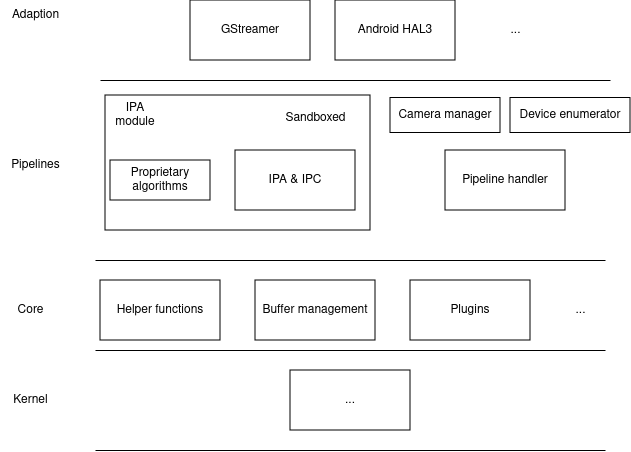
\includegraphics[width=0.60\textwidth]{figures/libcameraarch.png}
    \end{center}
    \caption{High level overview of how the libcamera architecture looks like}
    \label{fig:libcameraarch}
\end{figure}

libcamera\footnote{https://libcamera.org/} is an open-source C++ embedded
camera framework that supports a large number of complex cameras. Complex
cameras are cameras that require heavy hardware image processing, such as the
Sony IMX 219, 477 and many more. It supports multiple encoders to receive
images in for example PNGs/raw images. The primary target for libcamera is ARM
processors in the form of Raspberry PIs, Chromebooks and Android mobile phones
though many other architectures are also supported~\cite{libcameraStack}.
Because image processing algorithms are often proprietary and very secret,
libcamera also allows for binary blobs to be supplied by the vendors. The
vendors do need to submit the "base case" where the camera can take a still
image with decent quality to get the blob approved. These blobs are run in a
separate process, communicating with libcamera though an API provided by the
Pipeline Handler using \textit{dmabuf} handles. These \textit{dmabuf} handles
are very effective due to the fact that they do not require copies. If the user
wants to read the buffer, it can be mapped using \textit{mmap}. By default this
is not done, as mapping it would require the \textit{Memory Management Unit}
(MMU) to actually copy the data which requires work.

In \cref{fig:libcameraarch} we can see an overview of how libcamera looks like
from a birds eye view. libcamera provides buffer management along with a lot of
helper functions that allow the vendors to focus on what really matter; the
IPAs. The vendors are encouraged to open source the IPAs as maintaining a fork
is expensive. Additionally if the IPA is closed source there are some
restrictions: in order to ensure that the IPAs do not run any malicious code it
has a very limited access to the kernel, no network access, and a very
restricted view of the filesystem. Open source IPAs do not have these
restrictions, being verified by the maintainers that they do not have any
malicious code. Though as mentioned in the \cref{section:history} chapter,
there are "smart sensors" where the sensor itself has an integrated ISP. These
do not require IPAs and can instead be used as is. IPAs are only required when
the ISP is controlled by the CPU~\cite{libcameraStack}.

One of libcameras most critical functionalities is its high-level interface
for capturing images and videos. This interface allows applications to
interact with cameras using frameworks like \textit{GStreamer}, simplifying
building pipelines for media processing. The capture process in libcamera
follows a structured workflow:

First, before any operation, the camera must be acquired for exclusive access
using \textit{Camera::acquire}. This ensures that no other process can interfere with
capturing operations\footnote{\href{https://libcamera.org/api-html/classlibcamera_1_1Camera.html\#a4e60f8015f64e5897394d6677e3fb274}{Camera::acquire}}.
Once acquired, the camera needs to be configured according to the desired
capture parameters (e.g., resolution, format) using \textit{Camera::configure}, where
developers define which streams will be involved in capturing and how they
should be configured\footnote{\href{https://libcamera.org/api-html/classlibcamera_1_1Camera.html\#a4c190f4c369628e5cd96770790559a26}{Camera::configure}}.

After configuration, a request object is created using \textit{Camera::createRequest}.
This request holds buffers that will store captured frames\footnote{\href{https://libcamera.org/api-html/classlibcamera_1_1Camera.html\#a5e5a9cdeef58daec5963b4715ecd4464}{Camera::createRequest}}.
The application fills these buffers with data before queuing them for capture.
With the request prepared, it is queued for processing using
\textit{Camera::queueRequest}. Once queued, libcamera handles the actual frame
capture and processes it according to the pipeline configuration\footnote{\href{https://libcamera.org/api-html/classlibcamera_1_1Camera.html\#a7017dfeac48e842d3e33c2c2eb217d62}{Camera::queueRequest}}.
When the capture completes, libcamera signals back to the application that the
request has been processed using callbacks. The application can then retrieve
and handle the captured data (e.g., saving it as an image file or passing it on
for further processing).

\subsection{HAL3 And Camera2}
\begin{figure}
    \begin{center}
        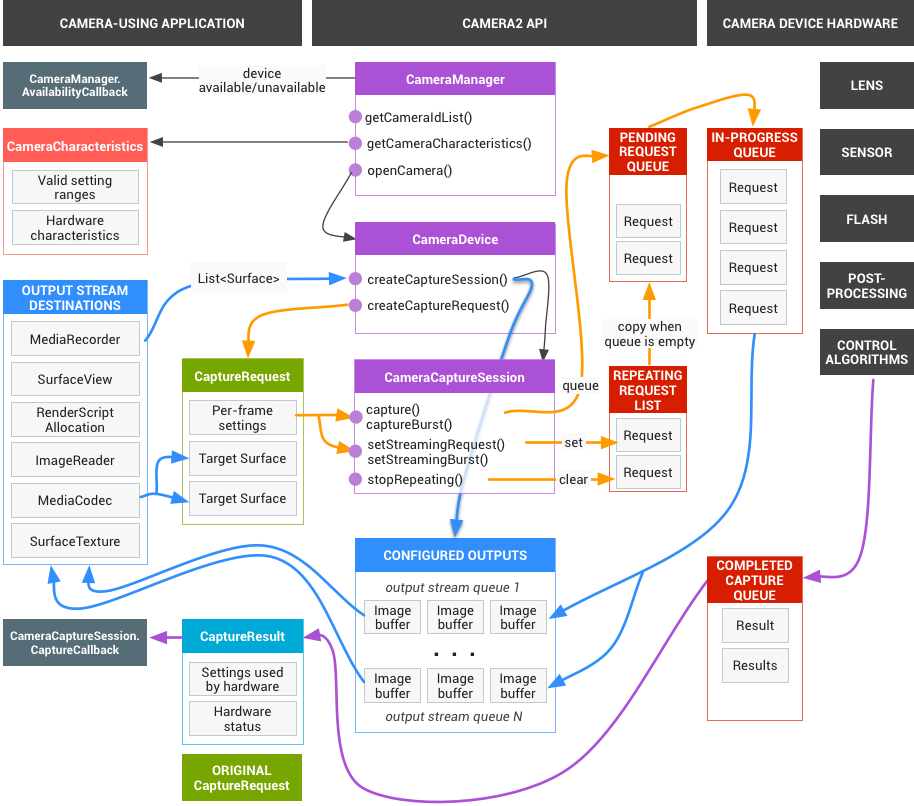
\includegraphics[width=0.90\textwidth]{figures/camera2.png}
    \end{center}
    \caption{Camera2 and HAL3 architecture,
    \textit{image source: https://source.android.com/docs/core/camera/camera3\_requests\_hal}}\label{fig:camera2}
\end{figure}


On Android, the camera system is structured around two primary APIs: the
Hardware Abstraction Layer 3\footnote{https://source.android.com/docs/core/camera/camera3} (HAL3)
and Camera2\footnote{https://developer.android.com/media/camera/camera2}. HAL3
is a low-level interface that provides the means for communicating with the
camera hardware and the Android framework, ensuring consistent interaction.
While HAL3 sits on roughly the same abstraction level as libcamera and Argus,
it is not made for the application developers to use. It is meant for camera
vendors to provide a unified way for Camera2 to communicate with the camera.

Camera2, however, is designed specifically for application developers. It
provides a higher-level interface that allows user-mode applications to
interact with the camera hardware, offering extensive control over camera
operations such as manual focus, exposure settings, and more. This makes
Camera2 ideal for developing complex camera applications. It provides a much
higher level view of a camera, comparable with for example Pipewire on Linux
providing a permission system and multiplexing.

HAL3 enhances app control over the camera subsystem while maintaining
efficiency by organizing operation modes into a unified view. It supports
various functionalities like burst mode, manual sensor control, and
post-processing features such as noise reduction and sharpening. This design
allows developers to create high-quality apps across different devices while
leveraging device-specific optimizations. The API models the camera as a
pipeline that processes requests for frame captures into frames on a 1:1 basis,
with each request including configuration details such as resolution and pixel
format.

Camera2 replaces the older Camera API by offering more granular control over
camera hardware through a pipeline model that processes capture requests in
sequence. This approach supports multiple requests simultaneously to maintain
full frame rates on most devices. With Camera2, developers can access detailed
camera characteristics, create capture sessions with customizable settings, and
implement features like auto-focus, RAW capture, and manual control over lens
and flash.

In \cref{fig:camera2} we can see how the pipeline works. It begins with the
application creating a CameraManager, which serves as the central interface for
accessing all available camera devices on the system. This manager provides a
list of CameraDevice instances, each representing a physical camera on the
device. Once a specific CameraDevice is selected, it is opened to create a
CameraCaptureSession in order to establish a connection with the camera
hardware. This step involves configuring the necessary settings and preparing
the device for capturing images or video. The application then creates
CaptureRequest objects, which define the parameters for each capture operation,
such as exposure settings, focus, and output targets like image buffers.

These capture requests are submitted to the CameraDevice through a
CaptureSession. This session manages the sequence of requests, ensuring they
are processed efficiently, whether in order or concurrently, based on the
applications requirements. The CameraDevice forwards each request to the HAL3,
which acts as an intermediary layer translating high-level requests into
specific hardware commands.

HAL3 communicates with the camera hardware, instructing it to perform tasks
such as adjusting lens focus or setting sensor exposure according to the
request parameters. The hardware then writes the captured data to designated
buffers within a buffer pool—pre-allocated memory spaces for temporary storage
of image data.

When processing is complete, the resulting image data is available in these
buffers for retrieval. The application can access this data for further
processing or display purposes. For each processed request, a CaptureResult
object is generated, containing metadata about the capture operation, such as
final exposure settings and focus distance. The application receives these
results through a callback mechanism, allowing it to handle captured images,
update user interface elements, or make adjustments for subsequent requests.
This pipeline not only ensures efficient handling of camera operations but also
provides developers with precise control over how images and videos are
captured on Android devices.


Despite its powerful tools, Camera2 introduces complexity due to
device-specific configurations and potential quirks across different Android
versions. To address these challenges, Google introduced CameraX\footnote{https://developer.android.com/media/camera/camerax},
a library designed to simplify camera app development by abstracting some of
these complexities and ensuring compatibility across devices. CameraX will not
be covered in this Thesis.

In conclusion, HAL3 serves as the foundational layer that ensures hardware
compatibility and performance optimization across devices. Building on this
foundation, Camera2 offers developers detailed control over camera features,
enabling the creation of sophisticated camera applications. Despite its
complexity, Camera2 remains essential for developers aiming to leverage
advanced camera capabilities in their apps.


\subsection{Kamaros}
Over the years there have been numerous camera standardization efforts such as
OpenKCam\footnote{https://www.khronos.org/openkcam}. However these have not been
successful due to lack of industry interest. Today the Khronos group has
started a push camera API standardization effort with \textit{Kamaros}\footnote{https://www.khronos.org/kamaros/}.

Kamaros is a new API currently being designed. Its goal is to
standardize embedded camera frameworks. This means that instead of needing
three different APIs for Android, L4T, Linux, and Windows you would only need to
use Kamaros. Allowing the applications to use a single API to communicate with
cameras over multiple platforms regardless of the platform. Though there are
still many other issues in the camera world that will not be solved by Kamaros.
Examples of these are for example camera configuration.

However, while Kamaros tries to address many of the current pain points in
embedded camera development, it is not without its limitations. One of the
biggest challenges in the camera world today is camera configuration.
Currently, there is no standardized way to configure cameras across different
platforms or devices. Camera drivers often make up a large portion of the
codebase because each driver is tailored to specific hardware. Despite this
complexity, many drivers share similar functionality but are implemented
differently due to the lack of standardization. Kamaros may attempt to tackle
this issue in future iterations by providing more standardized ways to
configure cameras, but this is not something that will be solved initially.

Another exciting aspect of Kamaros is its potential integration with Vulkan,
Khronoss low-overhead graphics and compute APIs. By leveraging Vulkan for
post-processing tasks, Kamaros could enable developers to take full advantage
of GPU acceleration for complex image processing tasks such as filtering,
noise reduction, or even real-time video processing. This would allow
developers to build highly efficient cross-platform applications without being
tied down by specific hardware or operating systems.

That said, Kamaros is still in its early stages of development, and much
remains unknown about its final form. The specification has not yet been
released, so it is difficult to comment on the specifics of how the API will
function or what features it will include at launch. However, based on
Khronoss track record with other successful standards like OpenGL and Vulkan,
there is reason to be optimistic about Kamaros's potential impact on the
embedded camera ecosystem.

\begin{figure}
    \begin{center}
        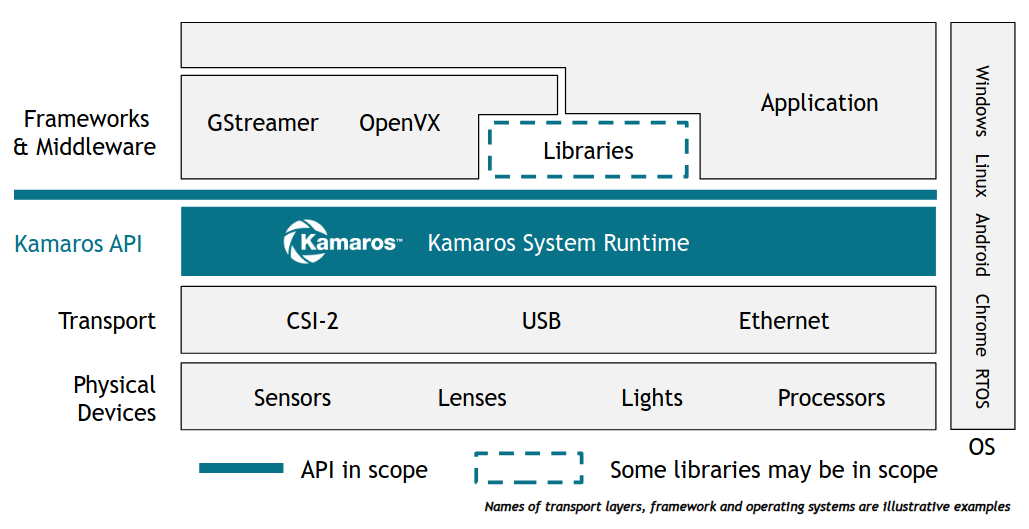
\includegraphics[width=0.60\textwidth]{figures/kamaros_stack.png}
    \end{center}
    \caption[Kamaros stack]{Kamaros stack, \textit{image source: \href{https://www.khronos.org/assets/uploads/developers/presentations/Khronos\_Kamaros\_Embedded\_World\_Mar23.pdf}{Embedded world}}}\label{fig:kamaros_stack}
\end{figure}

\subsection {GenICam}
Generic Interface for Cameras\footnote{\href{https://www.emva.org/wp-content/uploads/GenICam\_Standard\_v2\_1\_1.pdf}{GenICam Standard.pdf}} (GenICam),
is a standardized API developed by the European Machine Vision Association
(EMVA) to facilitate the integration and configuration of industrial cameras.
It provides a universal programming interface that decouples camera hardware
interfaces from user applications, allowing developers to work seamlessly with
different camera models and interfaces. This text will largely be based on the
GenICam standard.

A key feature of GenICam is its use of XML files to describe camera features
and settings, enabling self-describing cameras. This approach allows any
GenICam-compliant software to read and control cameras regardless of the
manufacturer or interface. While XML may not be as space-efficient as device
trees, it offers a flexible and standardized method for managing camera
configurations.

GenICam consists of several standardized modules that enhance its
functionality. The GenApi module defines a universal API for configuring
cameras using XML files, allowing manufacturers to provide machine-readable
manuals that map camera properties to registers. The Standard Features Naming
Convention (SFNC) ensures consistency in feature naming across different
devices, promoting interoperability. Additionally, the Generic Transport Layer
(GenTL) manages the transport of image data from the camera to the application,
supporting device enumeration and data streaming.

Widely adopted\footnote{https://www.emva.org/our-members/members/} in the
machine vision industry, GenICam supports various interfaces such as GigE
Vision, USB3 Vision, and CoaXPress. This broad compatibility facilitates
cross-manufacturer integration and reduces development time by eliminating the
need for camera-specific software. By providing a standardized interface,
GenICam simplifies the development process, reduces costs associated with
custom software development, and accelerates deployment times. It also ensures
compatibility and interoperability across different systems and applications.

As advancements in embedded systems continue, GenICam is poised to expand its
presence beyond traditional PC-based machine vision applications into embedded
environments\footnote{https://cdn.alliedvision.com/fileadmin/content/documents/products/cameras/various/appnote/CSI-2/GenICam-WhitePaper.pdf}.
This expansion offers flexibility and performance improvements
for industrial inspection and quality control tasks. Overall, GenICams
standardized approach significantly enhances the efficiency of developing
machine vision applications by providing a consistent framework for camera
control and data acquisition.

\subsection{Userspace}\label{section:userspace}
While not the focus of this thesis, a small introduction to how cameras should
be handled in userspace. In userspace most of these APIs can be used freely,
though they do often lock the camera, this means that only one application can
use the camera. In userspace this is often not enough, instead, we use some
multiplexing application or daemon such as Pipewire\footnote{https://pipewire.org/}.

Pipewire allows the user to set permissions for each application, enabling or
disabling the access to cameras. In the case of Pipewire, it builds on top of
libcamera and V4L2. Upon interviewing, some complaints were that Pipewire does
not have fine grained enough permission systems. They mention that a permission
system that would allow only access to specific cameras would be needed.
Currently it only allows for the application to either access them or not.

The interviews also suggested that the documentation is often not sufficient,
being difficult to decipher how things are done.

\section{API Comparison}\label{section:comparison}
\begin{table}
    \centering
    \begin{tabular}{|c|c|c|c|}
        \hline
        \thead{Feature} & \thead{Argus} & \thead{libcamera} & \thead{Android} \\ \hline
        AF &  & x & x \\ \hline
        AWB & x & x & x \\ \hline
        AGC & x & x & x \\ \hline
        Multi camera & x & x & x \\ \hline
        Partial images & x &  &  \\ \hline
        Open source &  & x & (x) \\ \hline
        License & Nvidia Copyright & LGPLv2.1 & AOSP licensing \\ \hline
        CUDA & x &  &  \\ \hline
        Platform & Tegra & Any Linux Machine & Android Systems \\ \hline
        HDR & x & x & x \\ \hline
        \makecell{Synchronized\\multi camera} & x &  &  \\ \hline
        OS support & L4T \& Android & Linux \& Android & Android \\ \hline
        Architecture & Request based & Request based & Request based \\ \hline
        Compression &  &  &  \\ \hline
        Raw image support & x & x & x \\ \hline
        Security &
        \makecell{Nvidia specific,\\receives additional\\safety measures\\from automotive} &
        \makecell{Linux system\\security configuration} &
        \makecell{Android\\security model} \\ \hline
        Supported cameras & >100 & 23 & Unknown \\ \hline
    \end{tabular}
    \caption{Feature comparison of camera APIs}
    \label{table:apiComparison}
\end{table}

While the APIs largely do the same thing, in a very similar fashion they still
have different use cases. Each still provide unique features when it comes to
both camera control, image processing, and the platforms they run on. In
\cref{table:apiComparison} we can see a full list of the feature comparison
done. Genicam is excluded in this comparison as it is completely dependent on
the vendor. The standard itself does not provide any functionality.

libcamera runs on essentially any platform that can run Linux, except for
Tegra devices running \textit{Linux For Tegra} (L4T). libcamera does not run
on L4T because the L4T V4L2 implementation has strayed too far from the
upstream version\footnote{https://github.com/kbingham/libcamera/issues/81} as
discussed in \cref{section:argus}.

When examining the various APIs, libcamera appears to be more accessible for
beginners. It offers straightforward examples for capturing images and requires
minimal setup. A notable example is the detailed explanation provided in its
documentation, which includes line-by-line commentary and illustrative ASCII
diagrams to elucidate hardware components\footnote{See \href{https://github.com/kbingham/simple-cam/blob/master/simple-cam.cpp}{simple-cam.cpp}}.
In contrast, the Android Camera2 API presents a more complex challenge due to
its extensive system requirements, necessitating comprehensive knowledge for
effective use and setup. Similarly, NVIDIA Argus provides powerful capabilities but
requiring a more extensive understanding of the ecosystem. There are a variety
of examples available on the device. These examples requires the user to buy
the device in order to view them.

One benefit that the Nvidia Argus has over other camera APIs, namely CUDA.
CUDA is a very popular way to program GPUs~\cite{kalaiselvi2017survey}, this
puts gives Argus a unique standing where it supports CUDA very well. CUDA does
not support importing DMA buffers very well, this is because DMA symbols are
not exported to non GPL drivers\footnote{\href{https://github.com/torvalds/linux/blob/master/drivers/dma-buf/dma-buf.c}{dma-buf.c}}
which means that libcamera does not properly support CUDA. This means that
Nvidia drivers are not able to properly utilize the feature, which in turn also
has a negative side effect where libcamera gives DMA buffers to the user, CUDA
can not import them. There was an effort in 2012 to make DMA symbols exported
to non-GPL code\footnote{\href{https://patchwork.kernel.org/project/dri-devel/patch/1349884592-32485-1-git-send-email-rmorell@nvidia.com/}{Mailing
list}} though it did not get approved. The other APIs can use Vulkan compute
which is a similar system as CUDA, it is open-source and maintained by the
Khronos group.

Stereo camera support is currently only offered by Argus, the allow
to time the capture requests very closely and measure when they were captured.
Genicam has varying support for this, though as previously mentioned, it is very
vendor specific and the manual must be referenced to see if it is. Camera2 and
libcamera have support for multi camera use cases, though they do not have the
synchronization support necessary.

While the APIs do not directly support encoding YUV images to for example JPEG
directly. This process is often not very difficult for the user to implement
using dedicated libraries such as jpeglib or NvJPEGEncoder that enable JPEG
creation, a sample for jpeglib can be found in the Raspberry Pi apps
tree\footnote{https://github.com/raspberrypi/rpicam-apps/blob/main/apps/rpicam\_jpeg.cpp}.

